\documentclass[11pt,reqno]{amsart}

\usepackage{amsthm,amsmath,amssymb}
\usepackage{mathtools}
\usepackage{proof}
\usepackage{xcolor}
\usepackage{graphicx}
\usepackage[T1]{fontenc}
\usepackage{courier}
\usepackage{hyperref}
\hypersetup{
    hidelinks=true
}
\usepackage{array}
\usepackage{multirow}
\usepackage{listings}
\lstset{basicstyle=\ttfamily\tiny, columns=fullflexible, language=Python, morekeywords={logical_and, log, exp, dot, sqrt, ones, identity}}
\newcommand{\code}[1]{\texttt{#1}}
\newcommand\MyBox[2]{
  \fbox{\lower0.75cm
    \vbox to 1.7cm{\vfil
      \hbox to 1.7cm{\hfil\parbox{1.4cm}{#1\\#2}\hfil}
      \vfil}%
  }%
}
\graphicspath{ {./} }

\begin{document}

\begin{center}
\large\textbf{Assignment 6 \\ DASC521 Fall 2019} \\
\normalsize\textbf{Introduction to Machine Learning \\  Erhan Tezcan 0070881 \\ 13.12.2019} \\
\end{center}

\section{Task}
We are given a dataset with number of cash withdrawals from 47 different ATMs of a bank using the information given about each ATM and the withdrawal date. A data entry has these information in order:
\begin{enumerate}
	\item ATM's identification number $id$
	\item ATM's geographical region $r \in \{1, 2, ..., 25\}$
	\item Transaction day $d$ as a number.
	\item Transaction month $m$ as a number.
	\item Transaction year $y$ as a number.
	\item Transaction type $t \in \{1, 2\}$: \begin{itemize}
		\item $1$: Card present
		\item $2$: No card present
		\end{itemize}
	\item Transaction count $c$ which is the number of cash withdrawals performed from the ATM with the given information. This is the output, and this is what we will try to predict.
\end{enumerate}
Unlike previous assignment, now we have a real-life machine learning problem on our hands. We are given the freedom of trying any method, as long as it works of course. Root mean squared error and mean absolute error will be our focus on evaluating our methods. Given the fact that our output variable is numeric, this is a regression problem with more than one feature.

\section{Implementation}
\subsection{Feature Selection}
First of all, on a problem like this it is important to check the features and correlations among eachother, most importantly the correlation between the feature and target output.
\begin{figure}[h]
	\centering
	\caption{Pearson Correlation Matrix}
	\label{cor}
	\begin{centering}
		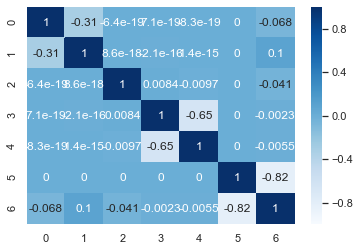
\includegraphics[width=0.7\textwidth]{cor.png}
	\end{centering}
\end{figure}
In figure \ref{cor} we have the Pearson Correlation Matrix. In that figure, 0 is $id$, 1 is $r$, 2 is $d$, 3 is $m$, 4 is $y$, 5 is $t$ and 6 is $c$. 
\subsubsection{Removing month and year features}
We can observe that month and year has very low correlation to the output variable. I have tried each method after removing month and year from the feature set, however, it performed worse. Thinking about the problem at hand, one may think that year does not have too much effect on the cash withdrawal unless the country is going through some ecomonic event at that year, but month would make a difference. I would like to say the low correlation surprised me at this. In the end, I have decided not to remove them from the feature set.
\subsubsection{Converting year, month and day to hours overall}
As another approach, I have tried to combine these 3 features into one by converting them to date and then calculating the hour difference between that date and epoch which is 1.1.1970. The results had more error, so I decided not to use this approach.
\subsubsection{Removing id feature}
Though id seems to have a correlation with the output variable, logically I found this to be slightly out of place. People dont choose a specific ATM usually, they choose whatever ATM is available and that is mostly defined by the region itself. Motivated by this, I have removed the id field and got better results immediately.
\subsubsection{Making region parameter dichotomous}
A known approach in categorical variables for regression is to convert the variable to many dichotomous (binary) variables. In the case of region, we have 31 different regions, so we will create 31 variables instead, where for example if a data row  $i$ has region $r=4$ then the corresponding variable will be 1, and every other region variable will be 0. In another words, we will do One-Hot-Encoding here. By itself, this performed worse, but combined with removing the id form features, this worked better overall. \\

In conclusion, I have converted region parameters to their respective dichotomous variables and removed the id feature. In the following subsections, I will describe my results with several methods, note that I am showing the results with the features removed. In my results, I will do 5-fold cross-validation and show the average errors, minimum and maximum errors from that cross-validation. I will also include the model training time (in seconds) on average.

\subsection{Decision Tree Regressor}
Due to its categorical independent variable nature, the first thing I tried was to try Decision Tree for regression. I have used \textit{sklearn.tree.DecisionTreeRegressor} from the \textit{sklearn} package. 
\begin{table}[]
\begin{tabular}{|c|l|l|l|}
\hline
Decision Tree & \multicolumn{1}{c|}{AVG} & \multicolumn{1}{c|}{MIN} & \multicolumn{1}{c|}{MAX} \\ \hline
\multicolumn{1}{|r|}{RMSE} & 24.92479 & 17.49900 & 32.08451 \\ \hline
\multicolumn{1}{|r|}{MAE} & 14.43111 & 10.42612 & 18.28205 \\ \hline
\multicolumn{4}{|l|}{Time (sec): 0.27629} \\ \hline
\end{tabular}
\caption{Decision Tree Regressor}
\label{tab:decisiontree}
\end{table}
The results are great! Good training time with kind of good error rates. Immediately, this gave me the motivation to research into decision tree regression techniques, and as a result I have 3 decision tree based methods in this task: Random Forest, XGBoost and LightGBM.

\subsection{Multilayer Perceptron Regressor}
I still wanted to try how a multilayer perceptron would perform in this task. My hyper parameters are:
\begin{itemize}
	\item Learning rate $0.01$
	\item 2 Hidden Layers, each of size 50.
	\item Alpha $0.001$
\end{itemize}
I have used \textit{sklearn.neural\_network.MLPRegressor} from \textit{sklearn} package.
\begin{table}[]
\begin{tabular}{|c|l|l|l|}
\hline
Multilayer Perceptron & \multicolumn{1}{c|}{AVG} & \multicolumn{1}{c|}{MIN} & \multicolumn{1}{c|}{MAX} \\ \hline
\multicolumn{1}{|r|}{RMSE} & 26.69785 & 21.82431 & 34.53084 \\ \hline
\multicolumn{1}{|r|}{MAE} & 15.80408 & 12.68853 & 19.84406 \\ \hline
\multicolumn{4}{|l|}{Time (sec): 8.82511} \\ \hline
\end{tabular}
\caption{Multilayer Perceptron Regressor}
\label{tab:mlp}
\end{table}
The first thing that catches the eye is the huge training time, which is expected given the nature of this algorithm. It also has the highest RMSE among the methods I have tried. So this is definetly not a good choice.

\subsection{XGBoost Regressor}
XGBoost stands for eXtreme Gradient Boosting. In general, Gradient Boosting is the practice of using an ensemble of trees (each having depth usually between 8 and 32) to predict the output variable. New models are created to deal with errors of existing models, and in the end you have an ensemble of models which you use together. XGBoost is one of the algorithms in this category of ``Boosted Gradients''. It is known for being fast and efficient. I have used \textit{xgboost} package.
\begin{table}[]
\begin{tabular}{|c|l|l|l|}
\hline
XGBoost & \multicolumn{1}{c|}{AVG} & \multicolumn{1}{c|}{MIN} & \multicolumn{1}{c|}{MAX} \\ \hline
\multicolumn{1}{|r|}{RMSE} & 26.12721 & 21.64978 & 32.44767 \\ \hline
\multicolumn{1}{|r|}{MAE} & 15.59602 & 12.76651 & 19.27959 \\ \hline
\multicolumn{4}{|l|}{Time (sec): 3.92292} \\ \hline
\end{tabular}
\caption{XGBoost Regressor}
\label{tab:xgboost}
\end{table}
Though it is known for being fast, we have a training time of 3.92292 on average, which we will is the slowest among the 4 methods I have tried, excluding multilayer perceptrons.

\subsection{Random Forest Regressor}
Random Forest is also an ensemble technique, but unlike boosters this one uses bagging. Bagging is when we use small samples of data to train and create many models (trees) and aggregate them in the end, hence the name: Forest. I have used \textit{sklearn.ensemble.RandomForestRegressor} by \textit{sklearn} package.
\begin{table}[]
\begin{tabular}{|c|l|l|l|}
\hline
Random Forest & \multicolumn{1}{c|}{AVG} & \multicolumn{1}{c|}{MIN} & \multicolumn{1}{c|}{MAX} \\ \hline
\multicolumn{1}{|r|}{RMSE} & 25.52983 & 23.22682 & 29.51543 \\ \hline
\multicolumn{1}{|r|}{MAE} & 15.74735 & 13.79042 & 17.89368 \\ \hline
\multicolumn{4}{|l|}{Time (sec): 0.16158} \\ \hline
\end{tabular}
\end{table}
Random Forest achieved the fastest training time, and a moderatly good error rate. However, we value the error rate more in this task, so this is still not the best choice.

\subsection{LightGBM Regressor}
Finally we have LightGBM, another Gradient Boosting framework, made by Microsoft. It is fast and accurate! I have used \textit{lightgbm} package.
\begin{table}[]
\begin{tabular}{|c|l|l|l|}
\hline
LightGBM & \multicolumn{1}{c|}{AVG} & \multicolumn{1}{c|}{MIN} & \multicolumn{1}{c|}{MAX} \\ \hline
\multicolumn{1}{|r|}{RMSE} & 24.64834 & 18.68125 & 32.22125 \\ \hline
\multicolumn{1}{|r|}{MAE} & 14.45761 & 10.89574  & 18.37656 \\ \hline
\multicolumn{4}{|l|}{Time (sec): 0.23766} \\ \hline
\end{tabular}
\end{table}
Decision Tree Regressor has a smaller MAE average error, but LightGBM has an even smaller RMSE error compared to Decision Tree Regressor, as well as slightly faster training time. As a result, I have decided to use LightGBM for this regression problem. Some hyper parameters I have are:
\begin{itemize}
	\item \textit{num\_leaves} $=34$. 
	\item \textit{learning\_rate} $=0.2$
	\item \textit{boosting\_type} as ``gbdt'' which stands for Gradient Boosting Decision Tree.
\end{itemize}
Note that one boosting type parameter was ``rf'' which stands for Random Forest, however it did not work so I used the Random Forest described in the previous subsection to test. The predictions stored in ``test\_predictions.csv'' are the results of lightGBM trained on the whole dataset. 


\end{document}